\documentclass[12pt,a4paper]{article}
\usepackage[a4paper,left=2cm,right=2cm,top=2cm,bottom=4cm]{geometry}
\usepackage[utf8]{inputenc}
\usepackage[T1]{fontenc}
\usepackage{amsmath}
\usepackage[ngerman]{babel}
\usepackage{amssymb}
\usepackage{float}
\usepackage{graphicx}
\usepackage{titling}
\usepackage{nicefrac}
\usepackage{xcolor}
\usepackage{nameref}
\definecolor{xsens}{RGB}{0,115,188}
\usepackage{sectsty}
\usepackage{inconsolata}
%\chapterfont{\color{xsens}}  % sets colour of chapters
%\sectionfont{\color{xsens}}  % sets colour of sections


%%%%%%%%%%%%%%%%%% HEADER AND FOOTER
\usepackage{fancyhdr}
\setlength\headheight{40pt}
\renewcommand{\headrulewidth}{0pt}
\pagestyle{fancy}
\lhead{\thetitle}
\rhead{
\includegraphics[height=4em]{Logos/X-SENSORS-Logo_Slogan_EN_Transparent.png}}
\rfoot{\thepage}
\cfoot{}

\usepackage{lipsum}

\author{Mirco Huber}
\newcommand{\subtitle}{Auswertung Vor-Ort-Messung auf Maschine}
\title{X-706: Vergleich zur aktuellen Serienlösung}
\begin{document}
	\begin{titlepage}
	\begin{figure}[H]
		\centering
		
\includegraphics[width=.5\linewidth]{Logos/X-SENSORS-Logo_Slogan_EN_Transparent.png}
	\end{figure}
	\vspace*{3cm}
	\begin{center}
		\Huge {\thetitle} \\\vspace*{.5cm}
		\small {\subtitle}
	\end{center}
	\vspace{12cm}
	\hspace{.6\linewidth} 
	\begin{tabular}{l}	
		\small{\theauthor} \\[.5pt]  
		\small{X-Sensors AG} \\ 
		\small{Landenbergerstrasse 13} \\
		\small{CH-8253 Diessenhofen} \\ [.5cm] 	
		\today
	\end{tabular}
\end{titlepage}
\section{Messkampagnenbeschreibung}
Für die Vergleichsmessung zwischen dem X-706 und dem GEFRAN SB46 wurde der X-706 (\texttt{P241126\_06}) neben dem Gefran-Sensor aufgeschraubt. Da das Bohrbild (4x M6) für die Befestigung des X-706 nachgebohrt werden musste und dabei ein Bohrer abgebrochen ist, wurde der X-706 für diese Versuchsreihe mit lediglich 3 Schrauben befestigt. Das Anzugsmoment betrug 14 Nm. Um die Lagetoleranzen der Befestigungslöcher etwas freier zu gestalten, wurden die Durchgangsbohrungen am X-706 von 6.2mm auf 6.5mm aufgebohrt.\\
\\
Der Messzyklus besteht aus folgenden Sequenzen:
\begin{enumerate}
	\item \label{it:opentara}Ruhephase mit nicht-vollständig geöffneter Form, während kein Tara-Signal an den Sensoren anliegt (0s bis ca. 1.9s)
	\item Vollständiges Öffnen der Form (ca. 2s bis 2.5s)
	\item Ruhephase mit anstehendem Reset / Tara = 1 (ca. 2.5s bis 6s)
	\item Schliessen der Form (ca. 6s bis 6.9s)
	\item Aufbringen der kompletten Schliesskraft (ca. 7s bis 8s)
	\item Öffnen der Form (ca. 8s bis 8.6s)
	\item Ruhephase  mit anstehendem Reset / Tara = 1 (ca. 8.6s bis 11s)
\end{enumerate} 
Der Signalverlauf ist in Abbildung \ref{fig:gesamtverlauf} dargestellt. Die Signale wurden direkt über die Maschinensteuerung mit einer Abtastrate von 1kHz aufgezeichnet.
\begin{figure}[H]
	\centering
	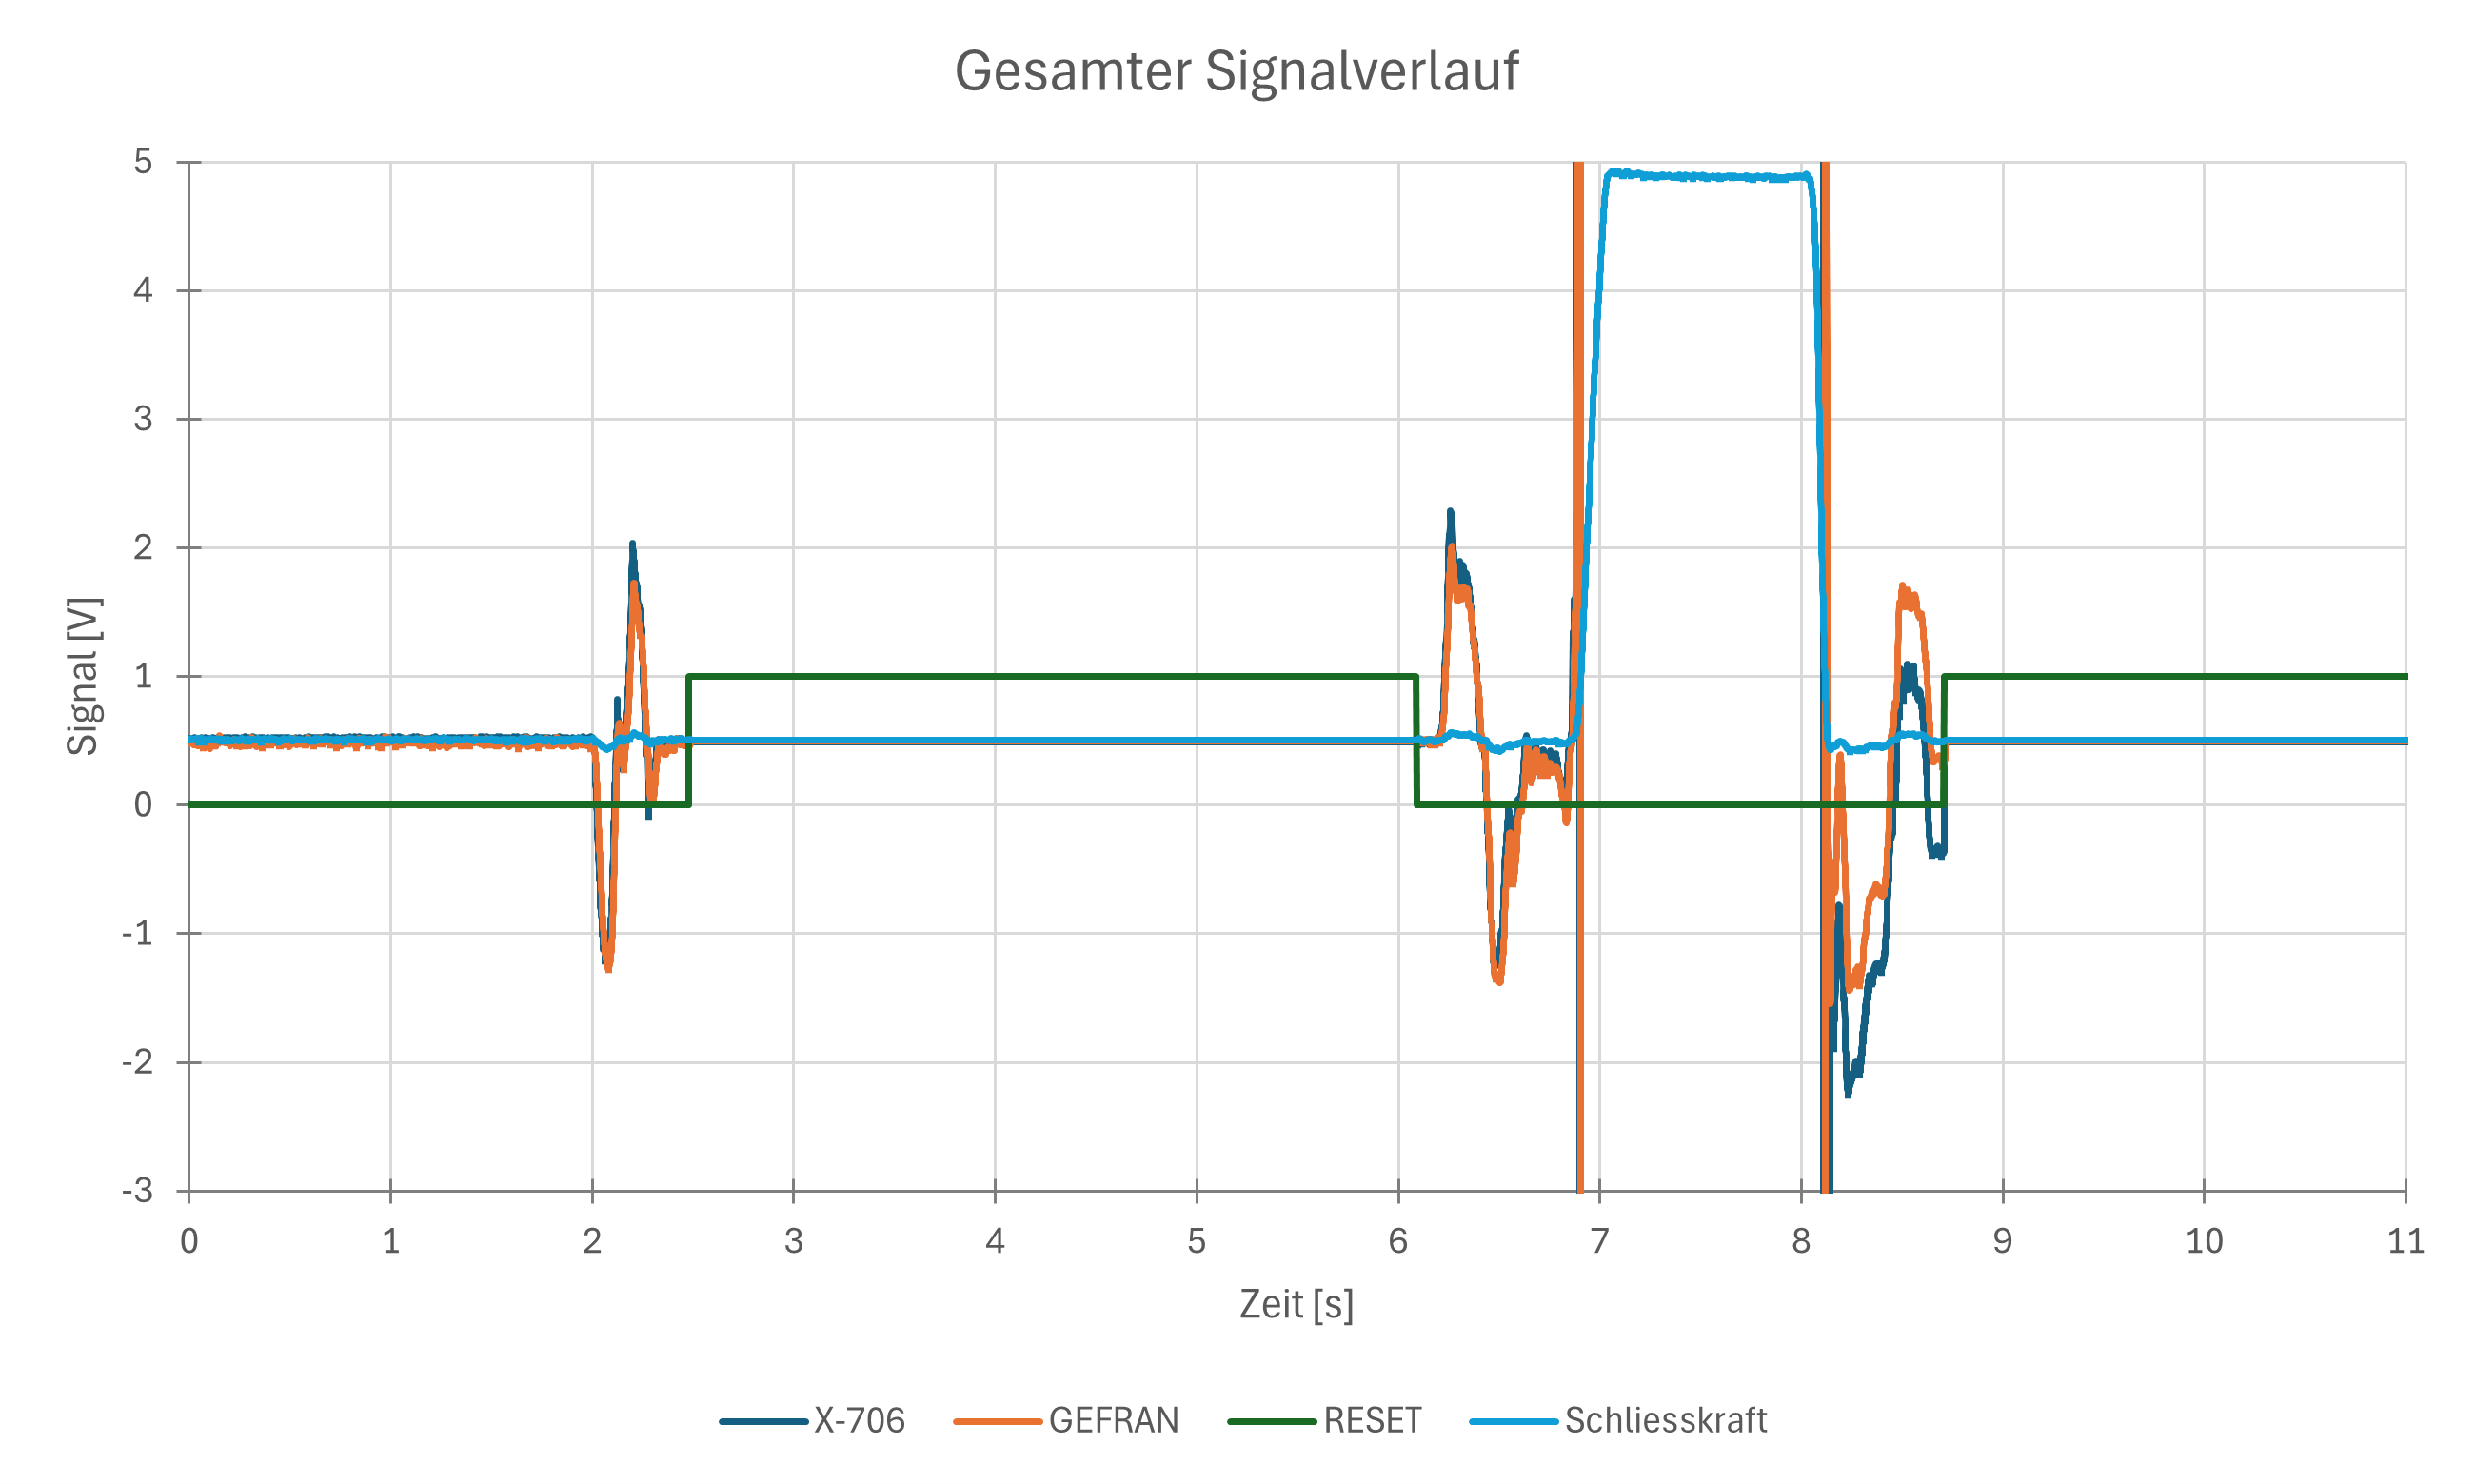
\includegraphics[width=1\linewidth]{imgs/Gesamtverlauf}
	\caption{Gesamter Signalverlauf}
	\label{fig:gesamtverlauf}
\end{figure}\noindent
Der Signalverlauf wird in den folgenden Abschnitten in die einzelnen Sequenzen aufgeteilt und genauer analysiert.
\section{Rauschverhalten in aufgeschraubtem Zustand; mit und ohne Tara}\label{sec:rauschen}
Im folgenden werden die Ausschnitte 1,3 und 7 detailierter betrachtet. Die Abschnitte zeigen das Rauschverhalten des aufgeschraubten Sensors mit anliegendem Tariersignal (3 und 7) sowie mit nicht-anliegendem Tariersignal.
\begin{figure}[H]
	\centering
	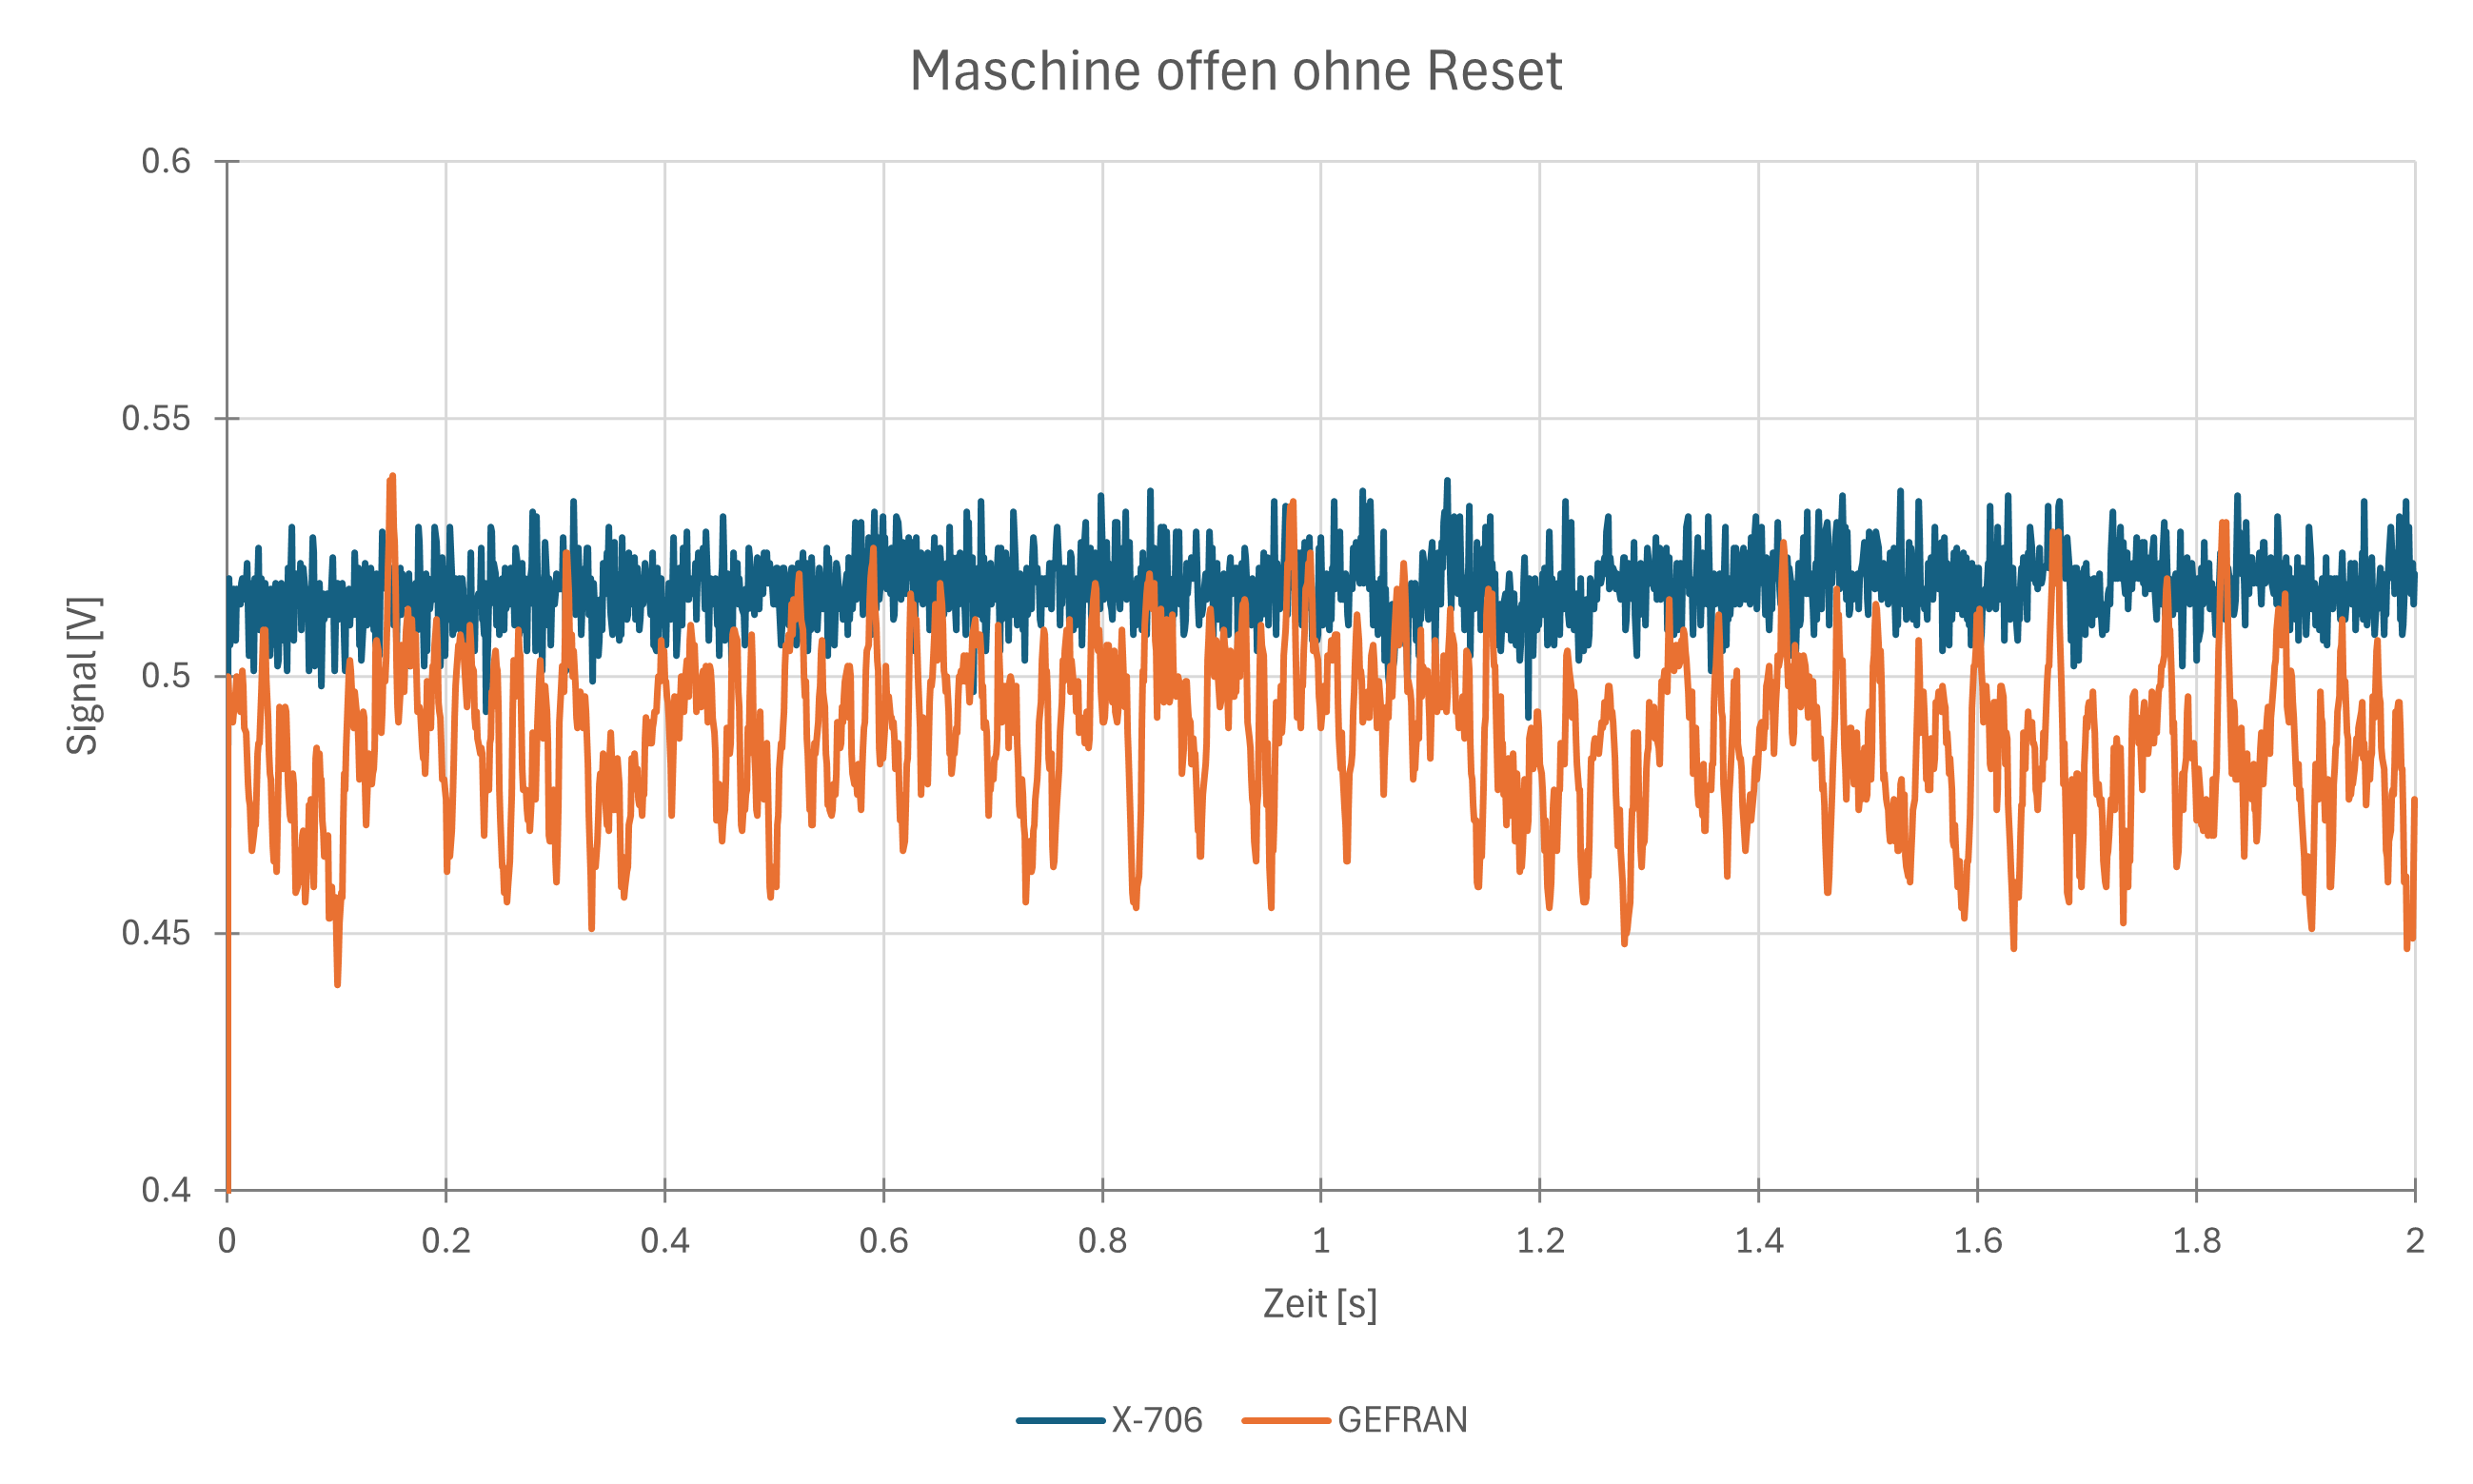
\includegraphics[width=1\linewidth]{imgs/rauschen_ohne_tara}
	\caption{Rauschverhalten bei Tara=0, Sequenz 1}
	\label{fig:rauschenohnetara}
\end{figure}\noindent
Die Abbildung \ref{fig:rauschenohnetara} \nameref{fig:rauschenohnetara} zeigt, dass das Signal des X-706 bei gelöstem Reset / Tara = 0 rauscharmer als als jenes des GEFRAN SB46. Weiter ist zu erkennen, dass beide Sensoren vergleichbar driften, wobei das Signal des X-706 näher am Tarierwert von 0.5V ist.\\
Liegt das Tariersignal an (Tara = 1, Sequenzen 3 und 7), fällt das Rauschen von beiden Sensoren gleich aus und liegt im Bereich von 1 LSB der Steuerungskarte. Das Tariersignal in Abbildung \ref{fig:rauschenmittara1} entspricht dem Signal vor dem kompletten Zyklus, das Signal in Abbildung \ref{fig:rauschenmittara1} entspricht jenem nach dem kompletten Zyklus (Schliessen, Schliesskraft aufbringe, Öffnen). Die Werte sind vor und nach dem Aufbringen der Schliesskraft bei beiden Sensoren identisch, was wiederum bedeutet, dass beide Sensoren die Überlast von ca. 350 $\mu\varepsilon$ verkraften.
\begin{figure}[H]
	\centering
	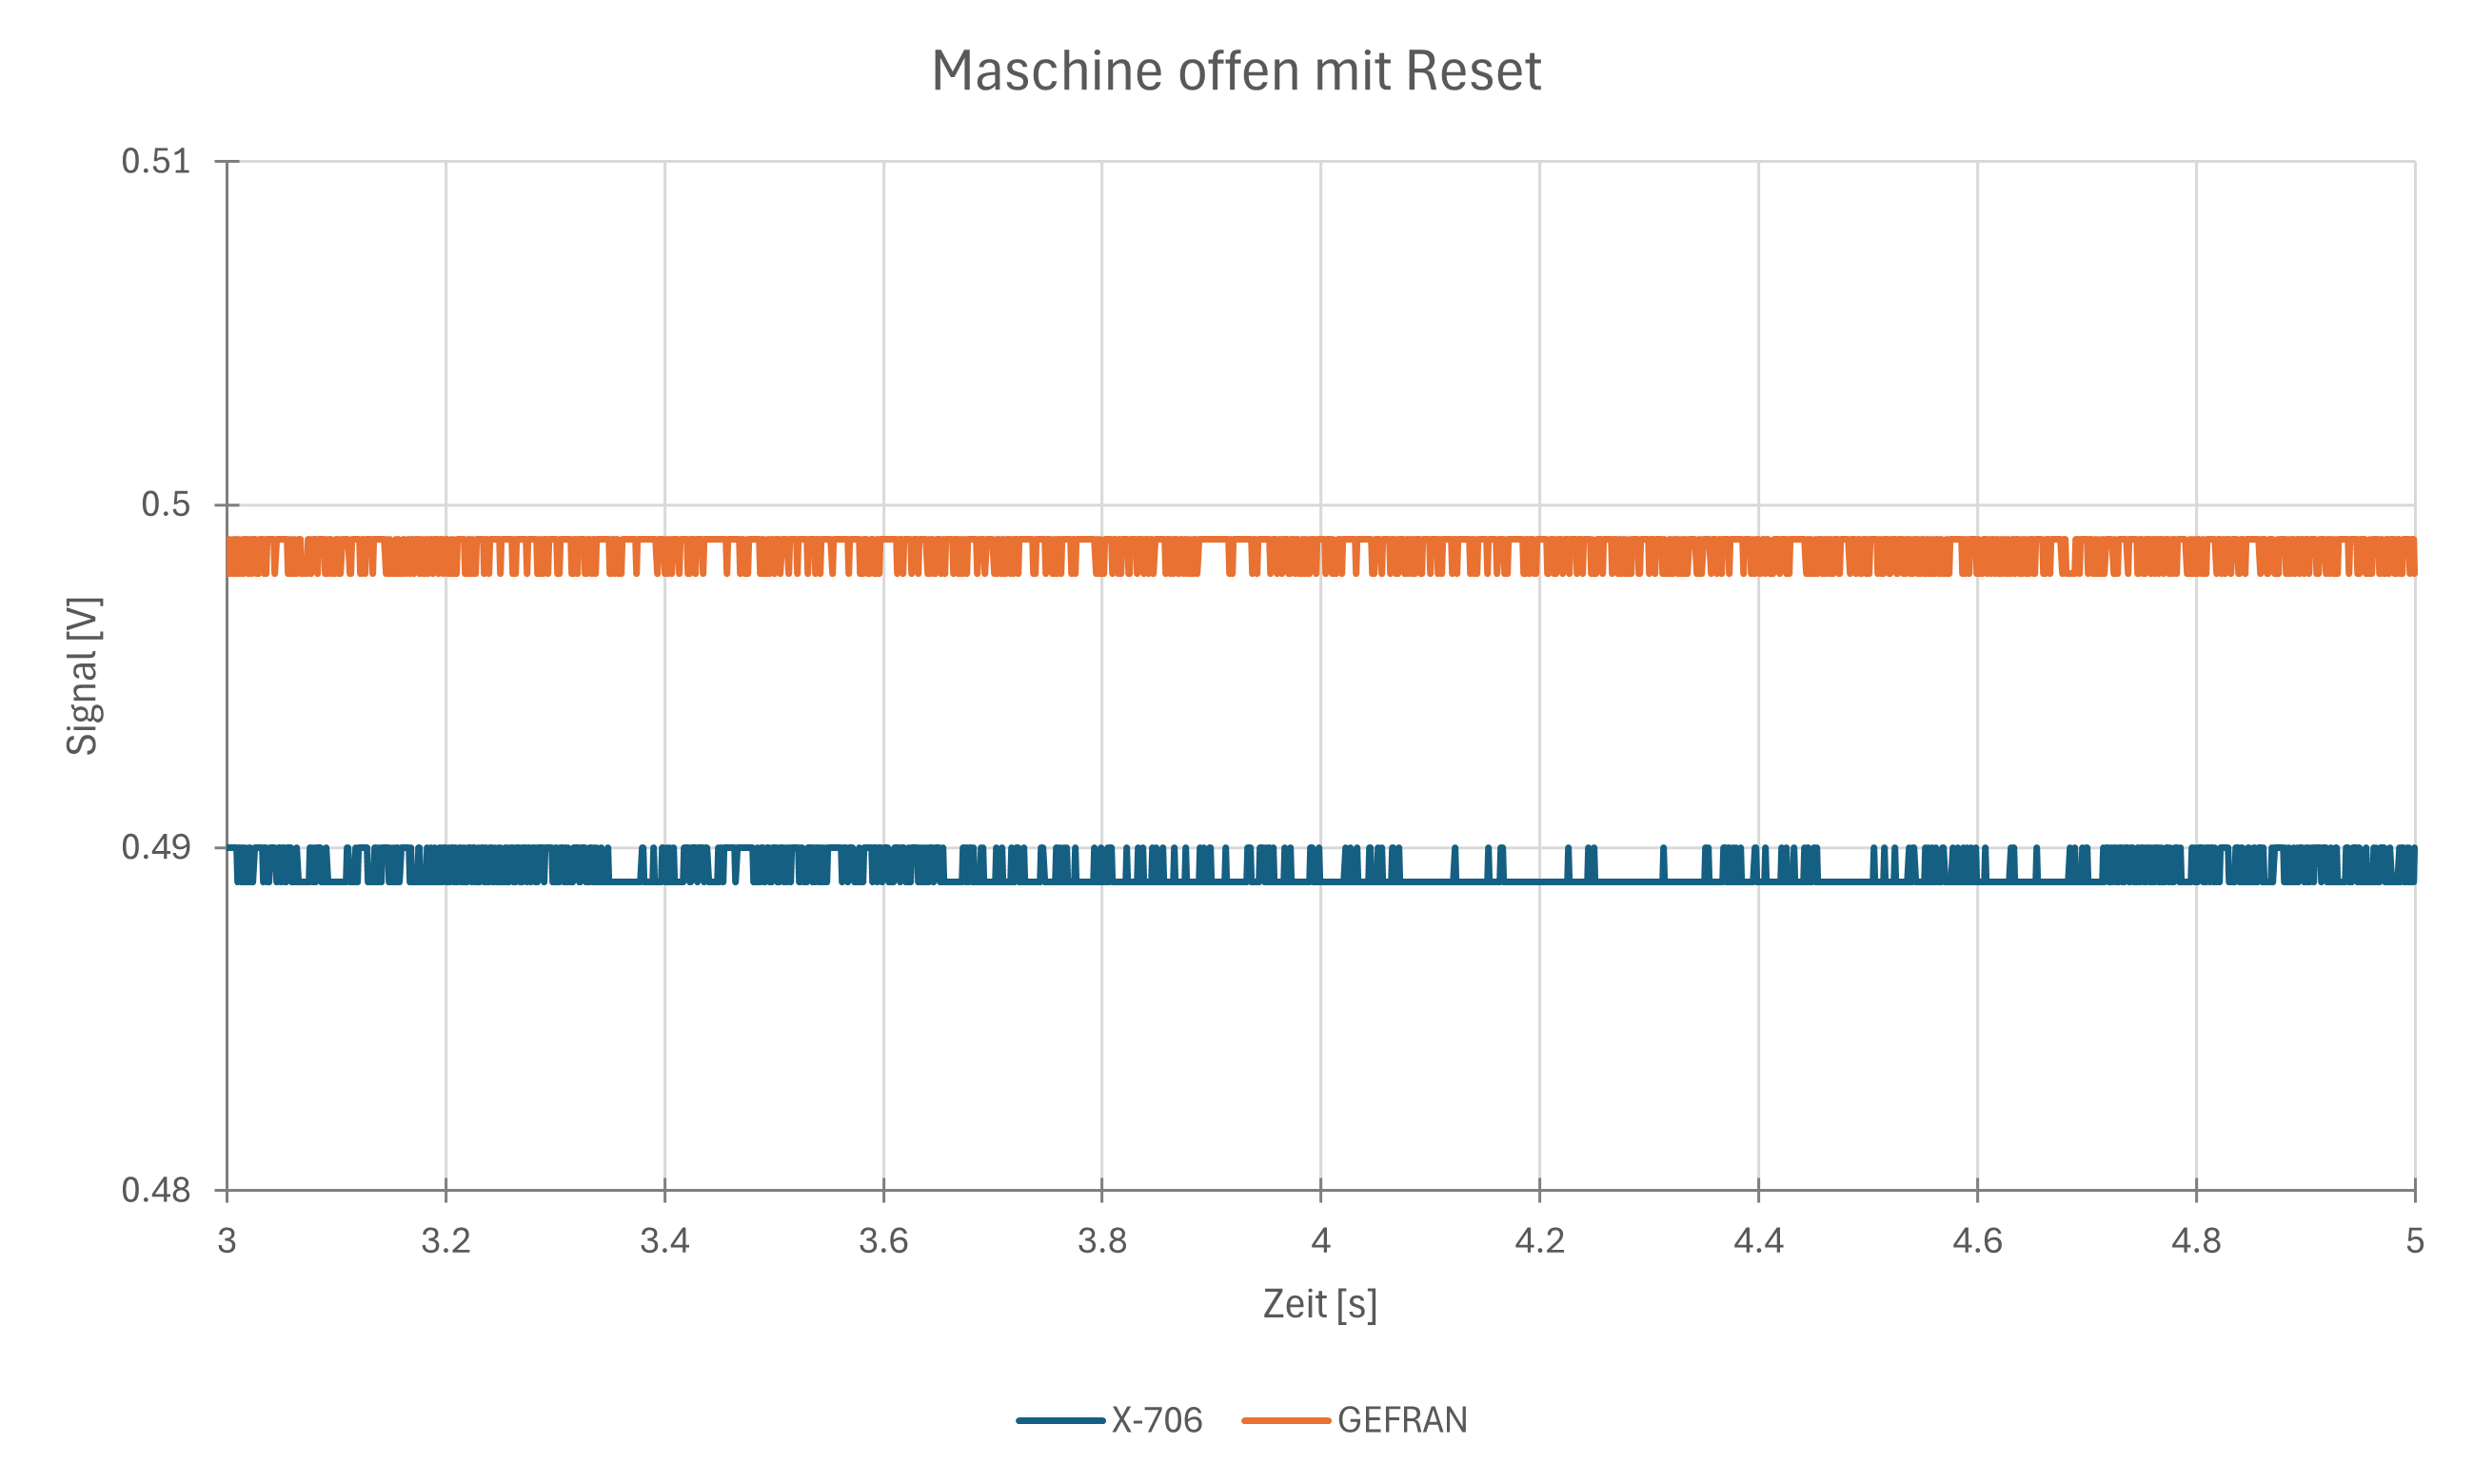
\includegraphics[width=1\linewidth]{imgs/rauschen_mit_tara1}
	\caption{Rauschverhalten bei Tara = 1}
	\label{fig:rauschenmittara1}
\end{figure}\noindent
Der Offset von rund 10mV des X-706 ist auf die Kalibrierung zurückzuführen. Die Kalibrierung erlaubt jedoch Schritte von 
\begin{equation*}
	\Delta U_{step}\frac{10V}{2.6}\cdot \frac{3}{2^{11}} \approx 5.6mV
\end{equation*}
was wiederum bedeutet, dass der Offset bei exakter Kalibration maximal $\pm\nicefrac{\Delta U_{step}}{2}$ und somit $\leq 2.8$mV beträgt.

\begin{figure}[H]
	\centering
	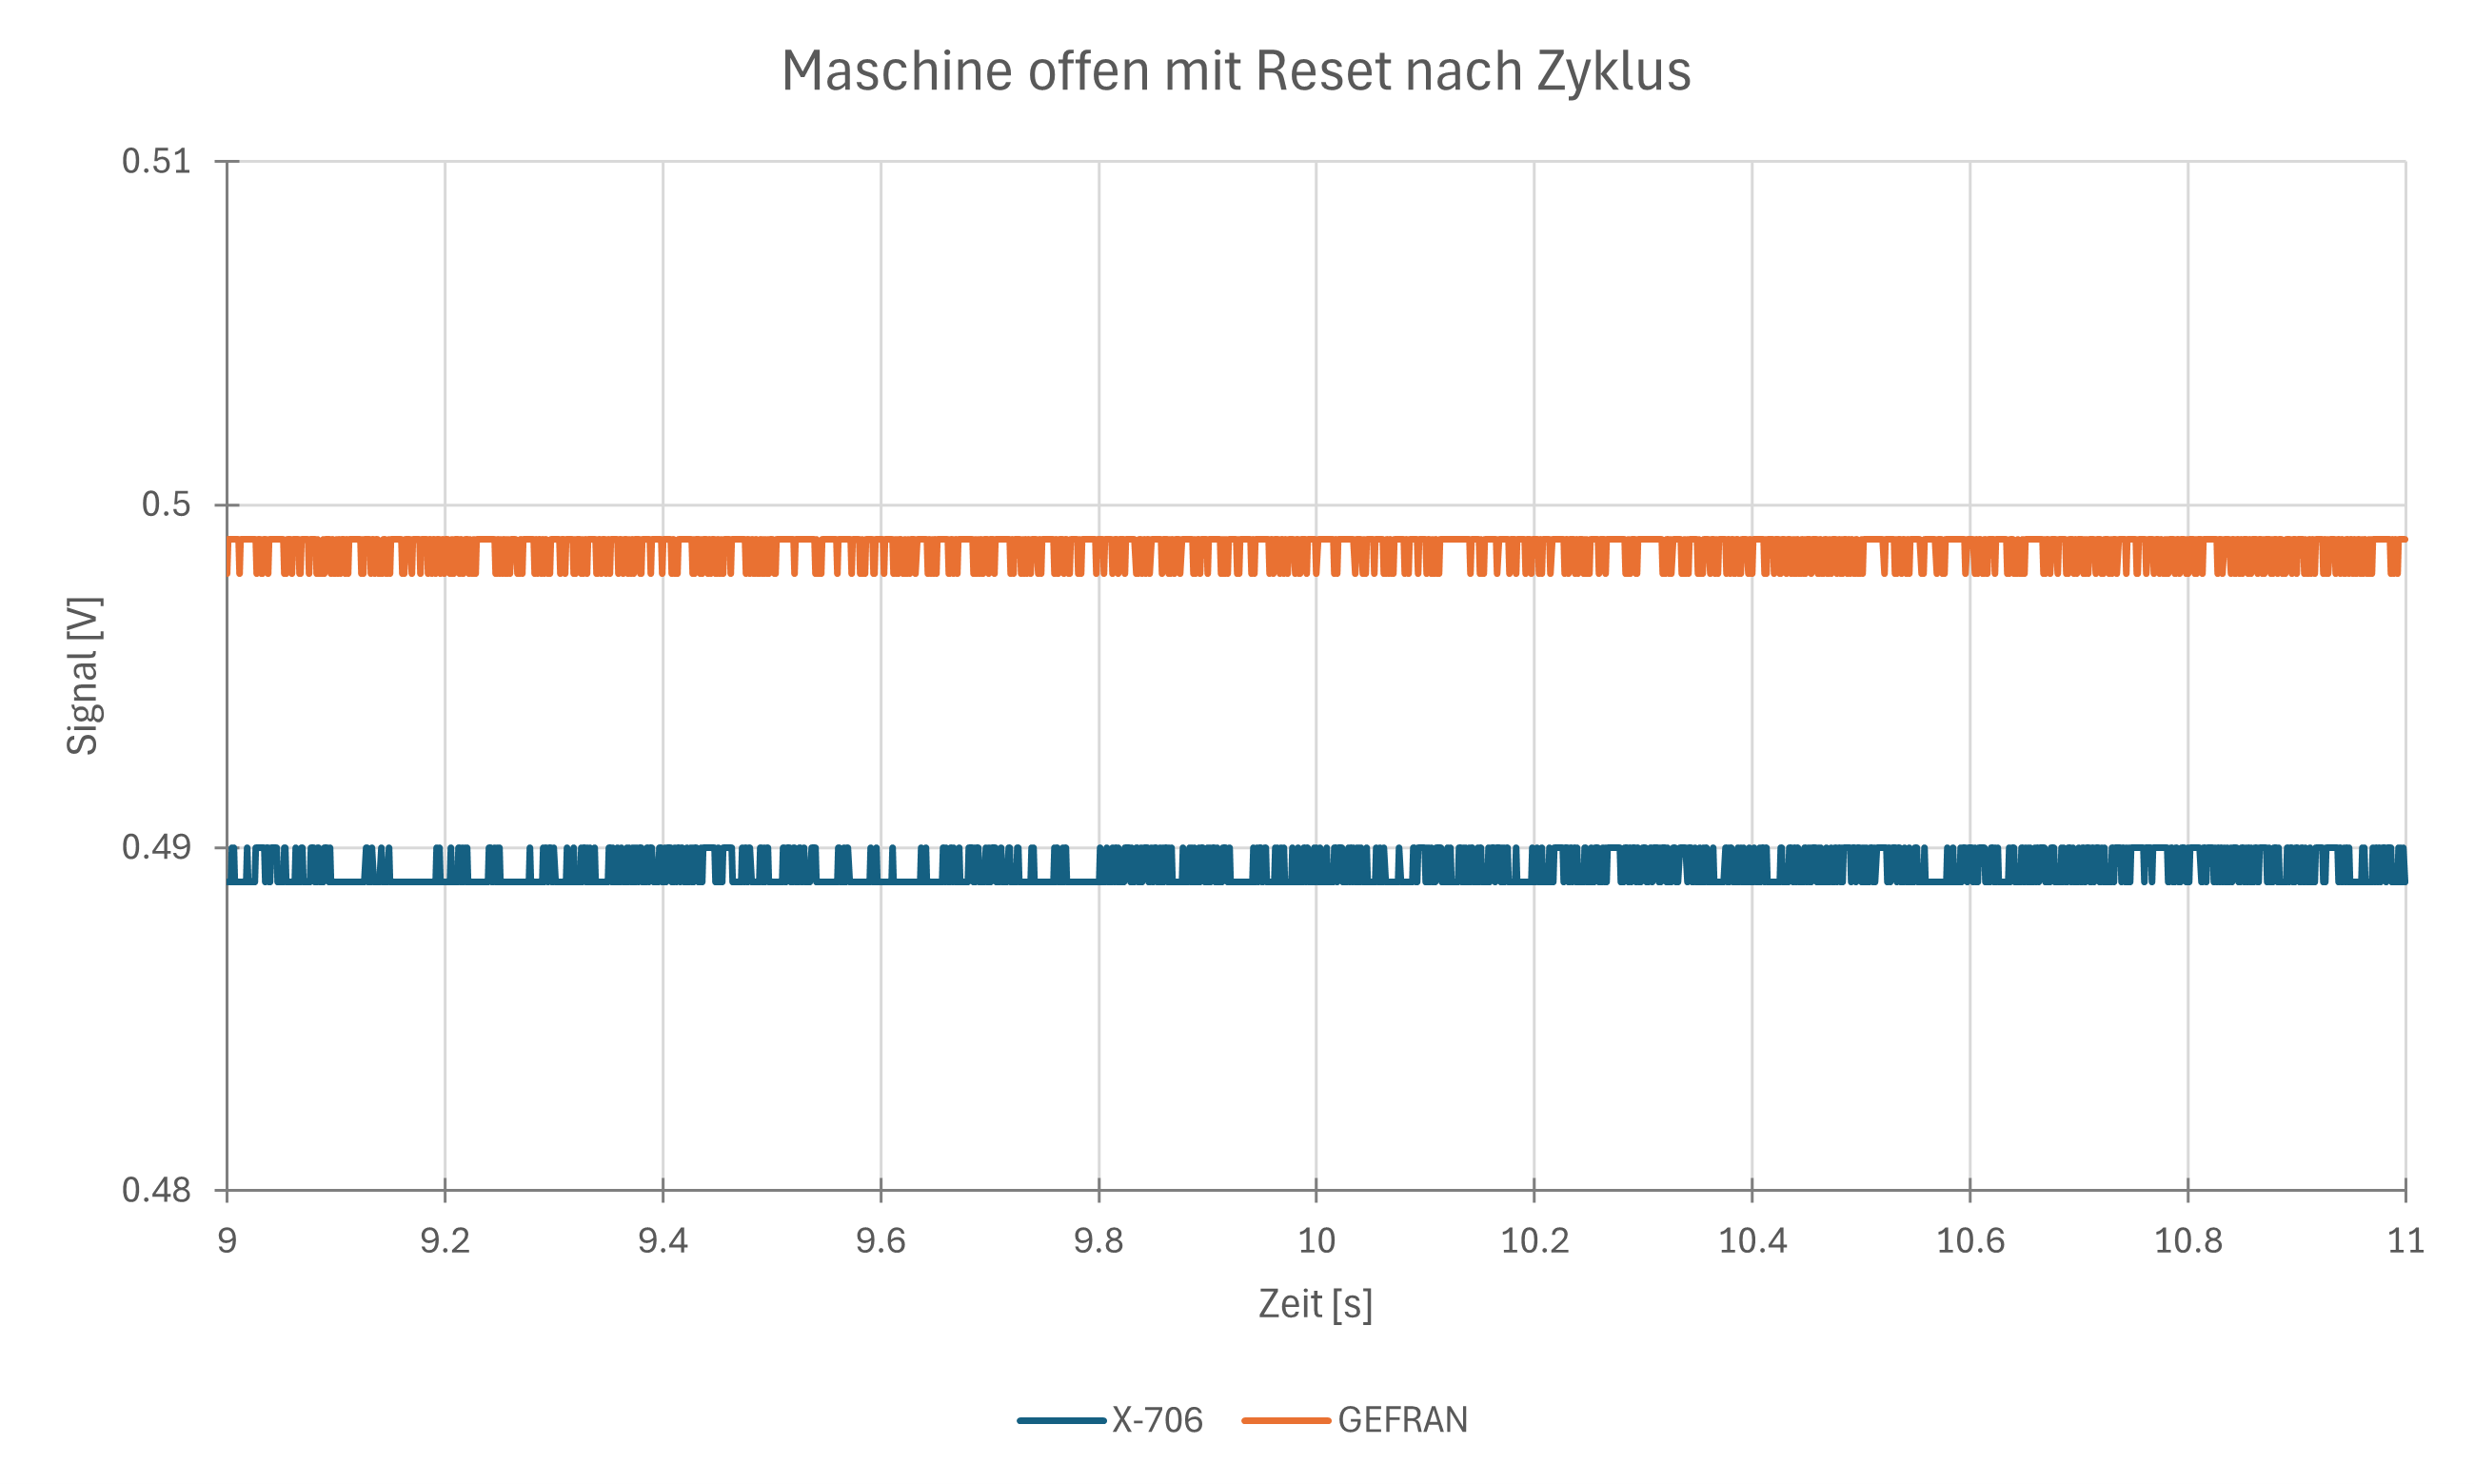
\includegraphics[width=1\linewidth]{imgs/rauschen_mit_tara2}
	\caption{Rauschverhalten bei Tara = 1 nach einem kompletten Zykuls inkl. Schliesskraft}
	\label{fig:rauschenmittara2}
\end{figure}
\section{Form Schliessen und Signallaufzeit}
Beim Signalverlauf während des Schliessvorgangs ist zu erkennen, dass der X-706 minim mehr Signal liefert und auch weniger stark glättet als der GEFRAN SB46. Durch das stärkere Glätten respektive die tiefere Eckfrequenz des Tiefpassfilters ist das Signal des GEFRAN-Sensors stärker verzögert als jenes des X-706. Der Signal-Verlauf ist aber bezüglich Spikes und Beträge nur bedingt vergleichbar, da die Sensoren nicht an der selben Stelle auf dem Kniehebel verbaut sind.
\begin{figure}[H]
	\centering
	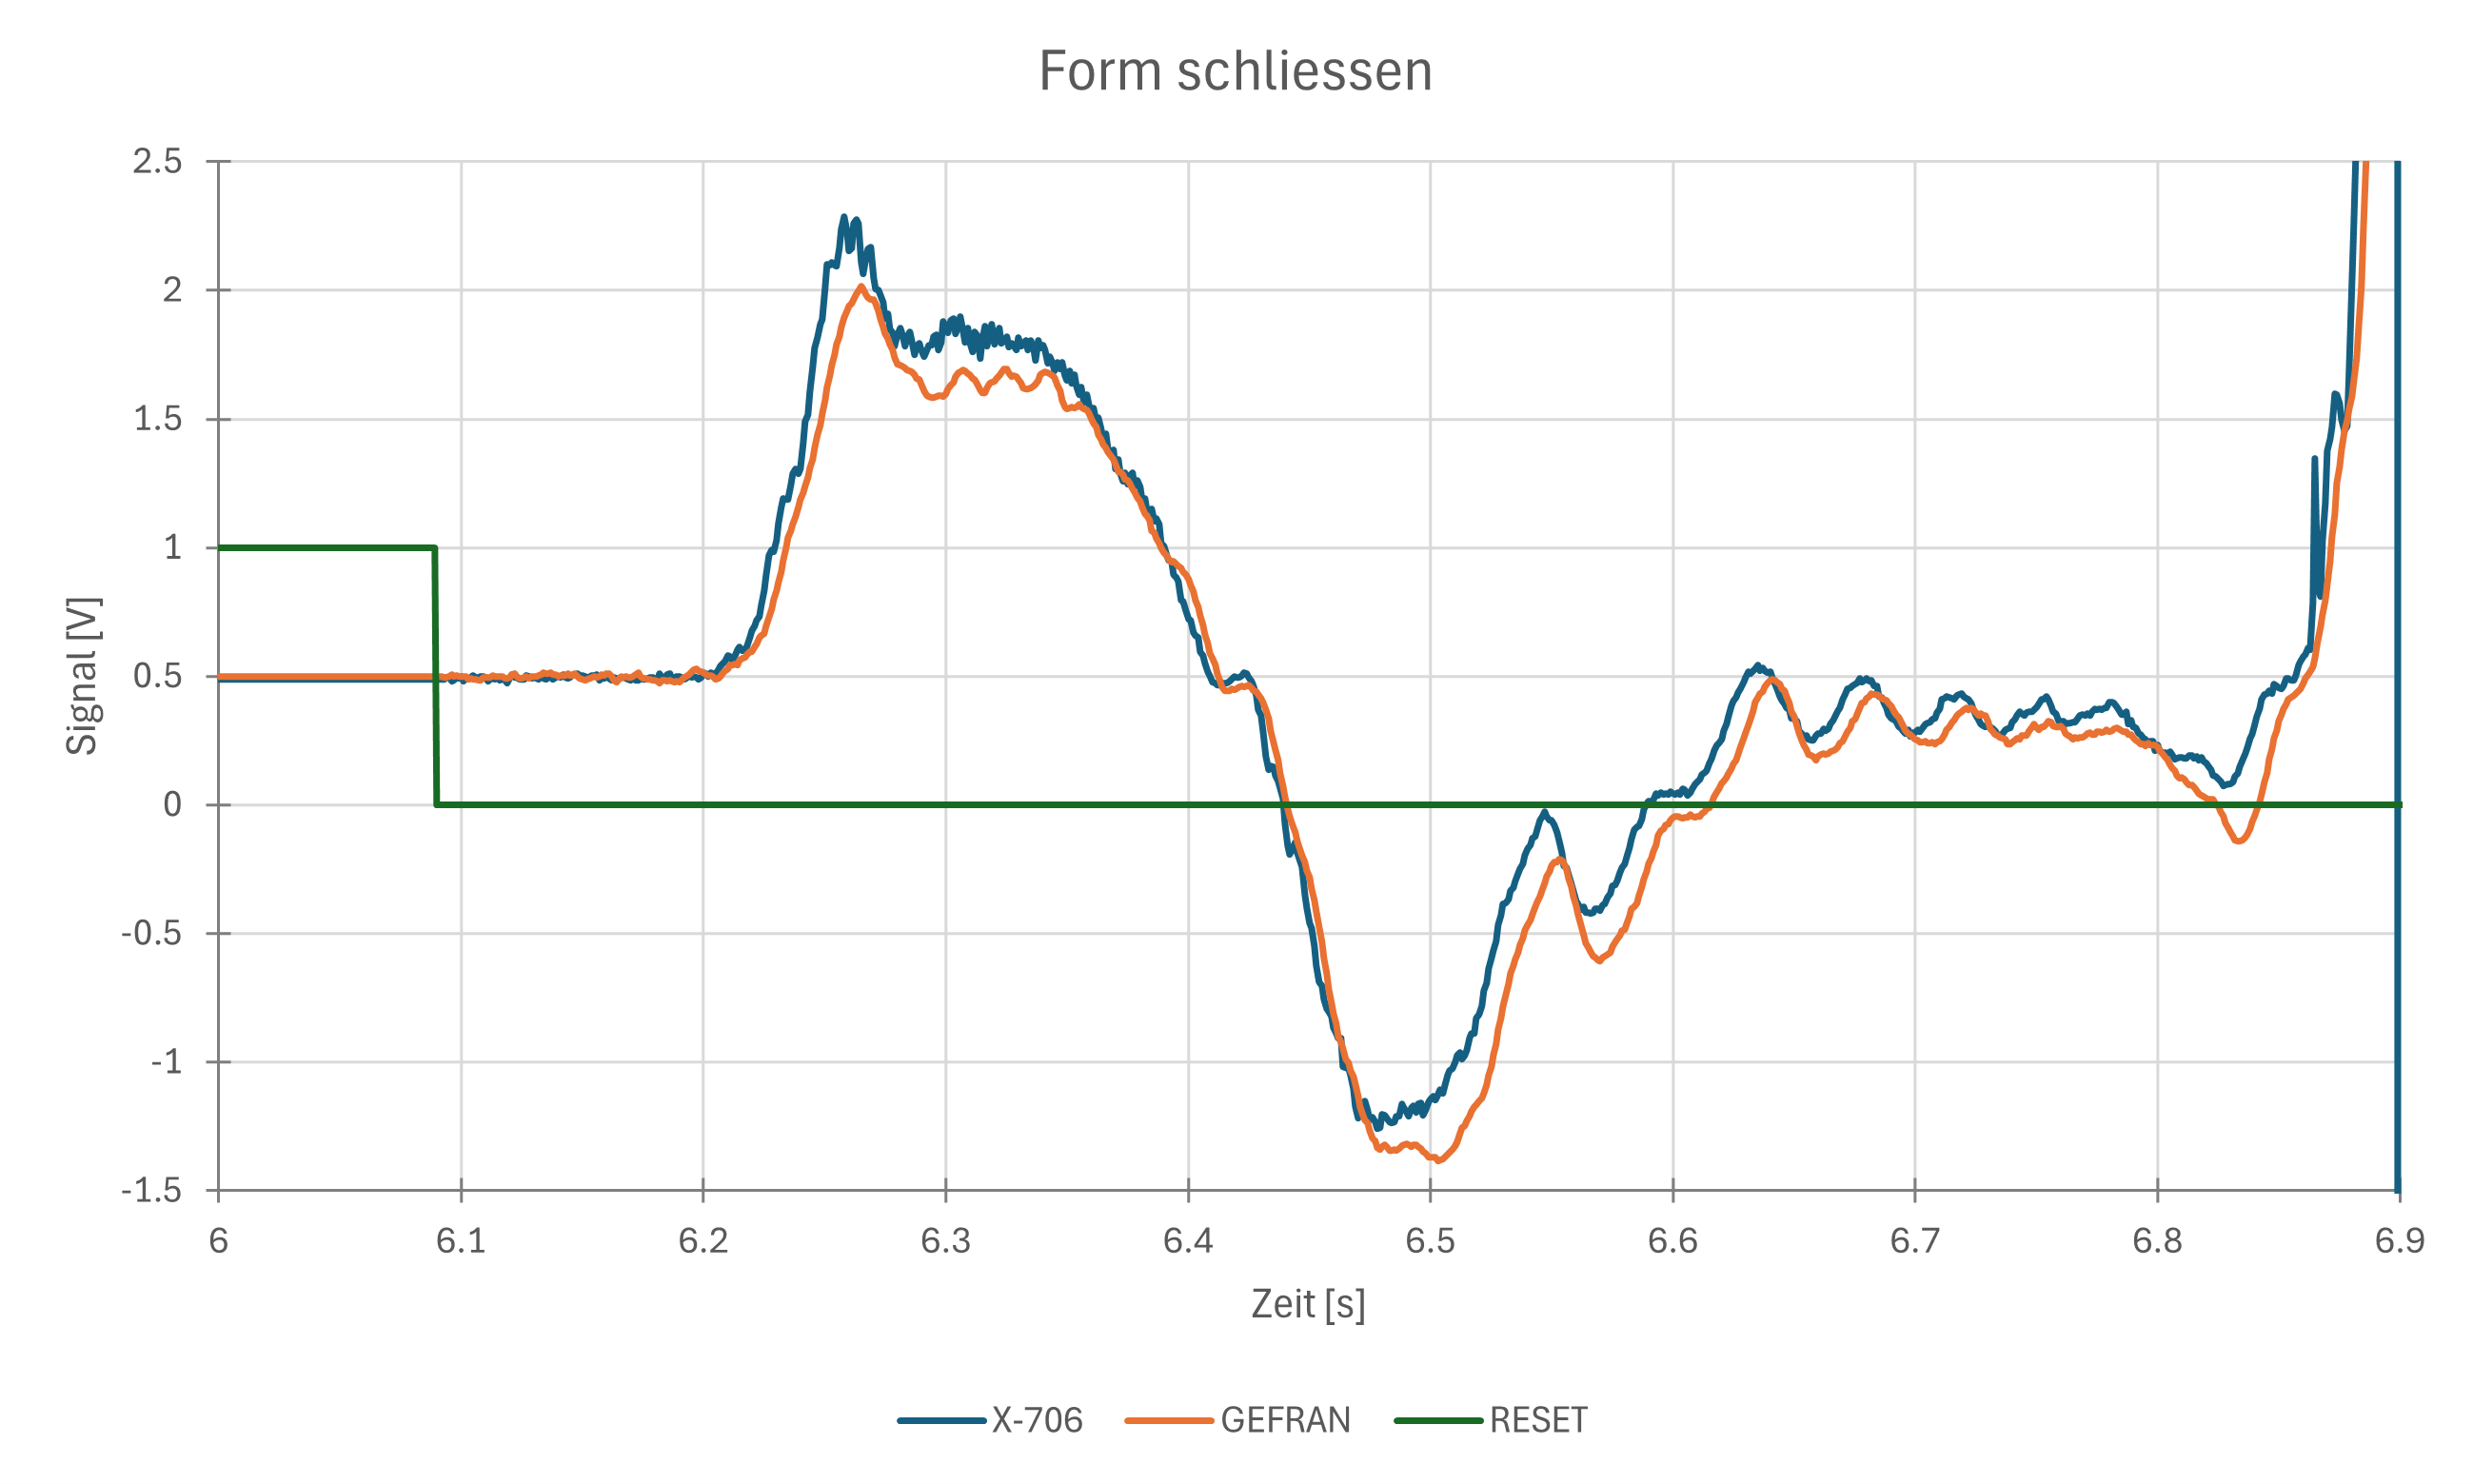
\includegraphics[width=1\linewidth]{imgs/form_schliessen}
	\caption{Signalverlauf beim Schliessen der Form}
	\label{fig:formschliessen}
\end{figure}\noindent
Dennoch lässt sich die schnellere Signallaufzeit auch beim ''\textit{Kabelbindertest}'' nachweisen, bei welchem die Maschine unter Verwendung des X-706-Signals minimal früher stoppt.
In obigem Signalausschnitt ist neben dem Schliessvorgang noch das Lösen des Resets (Übergang von Tara = 1 auf Tara = 0) zu sehen. Dieser Ausschnitt ist in Abbildung \ref{fig:taraloesen} noch detailierter visualisiert.
\begin{figure}[H]
	\centering
	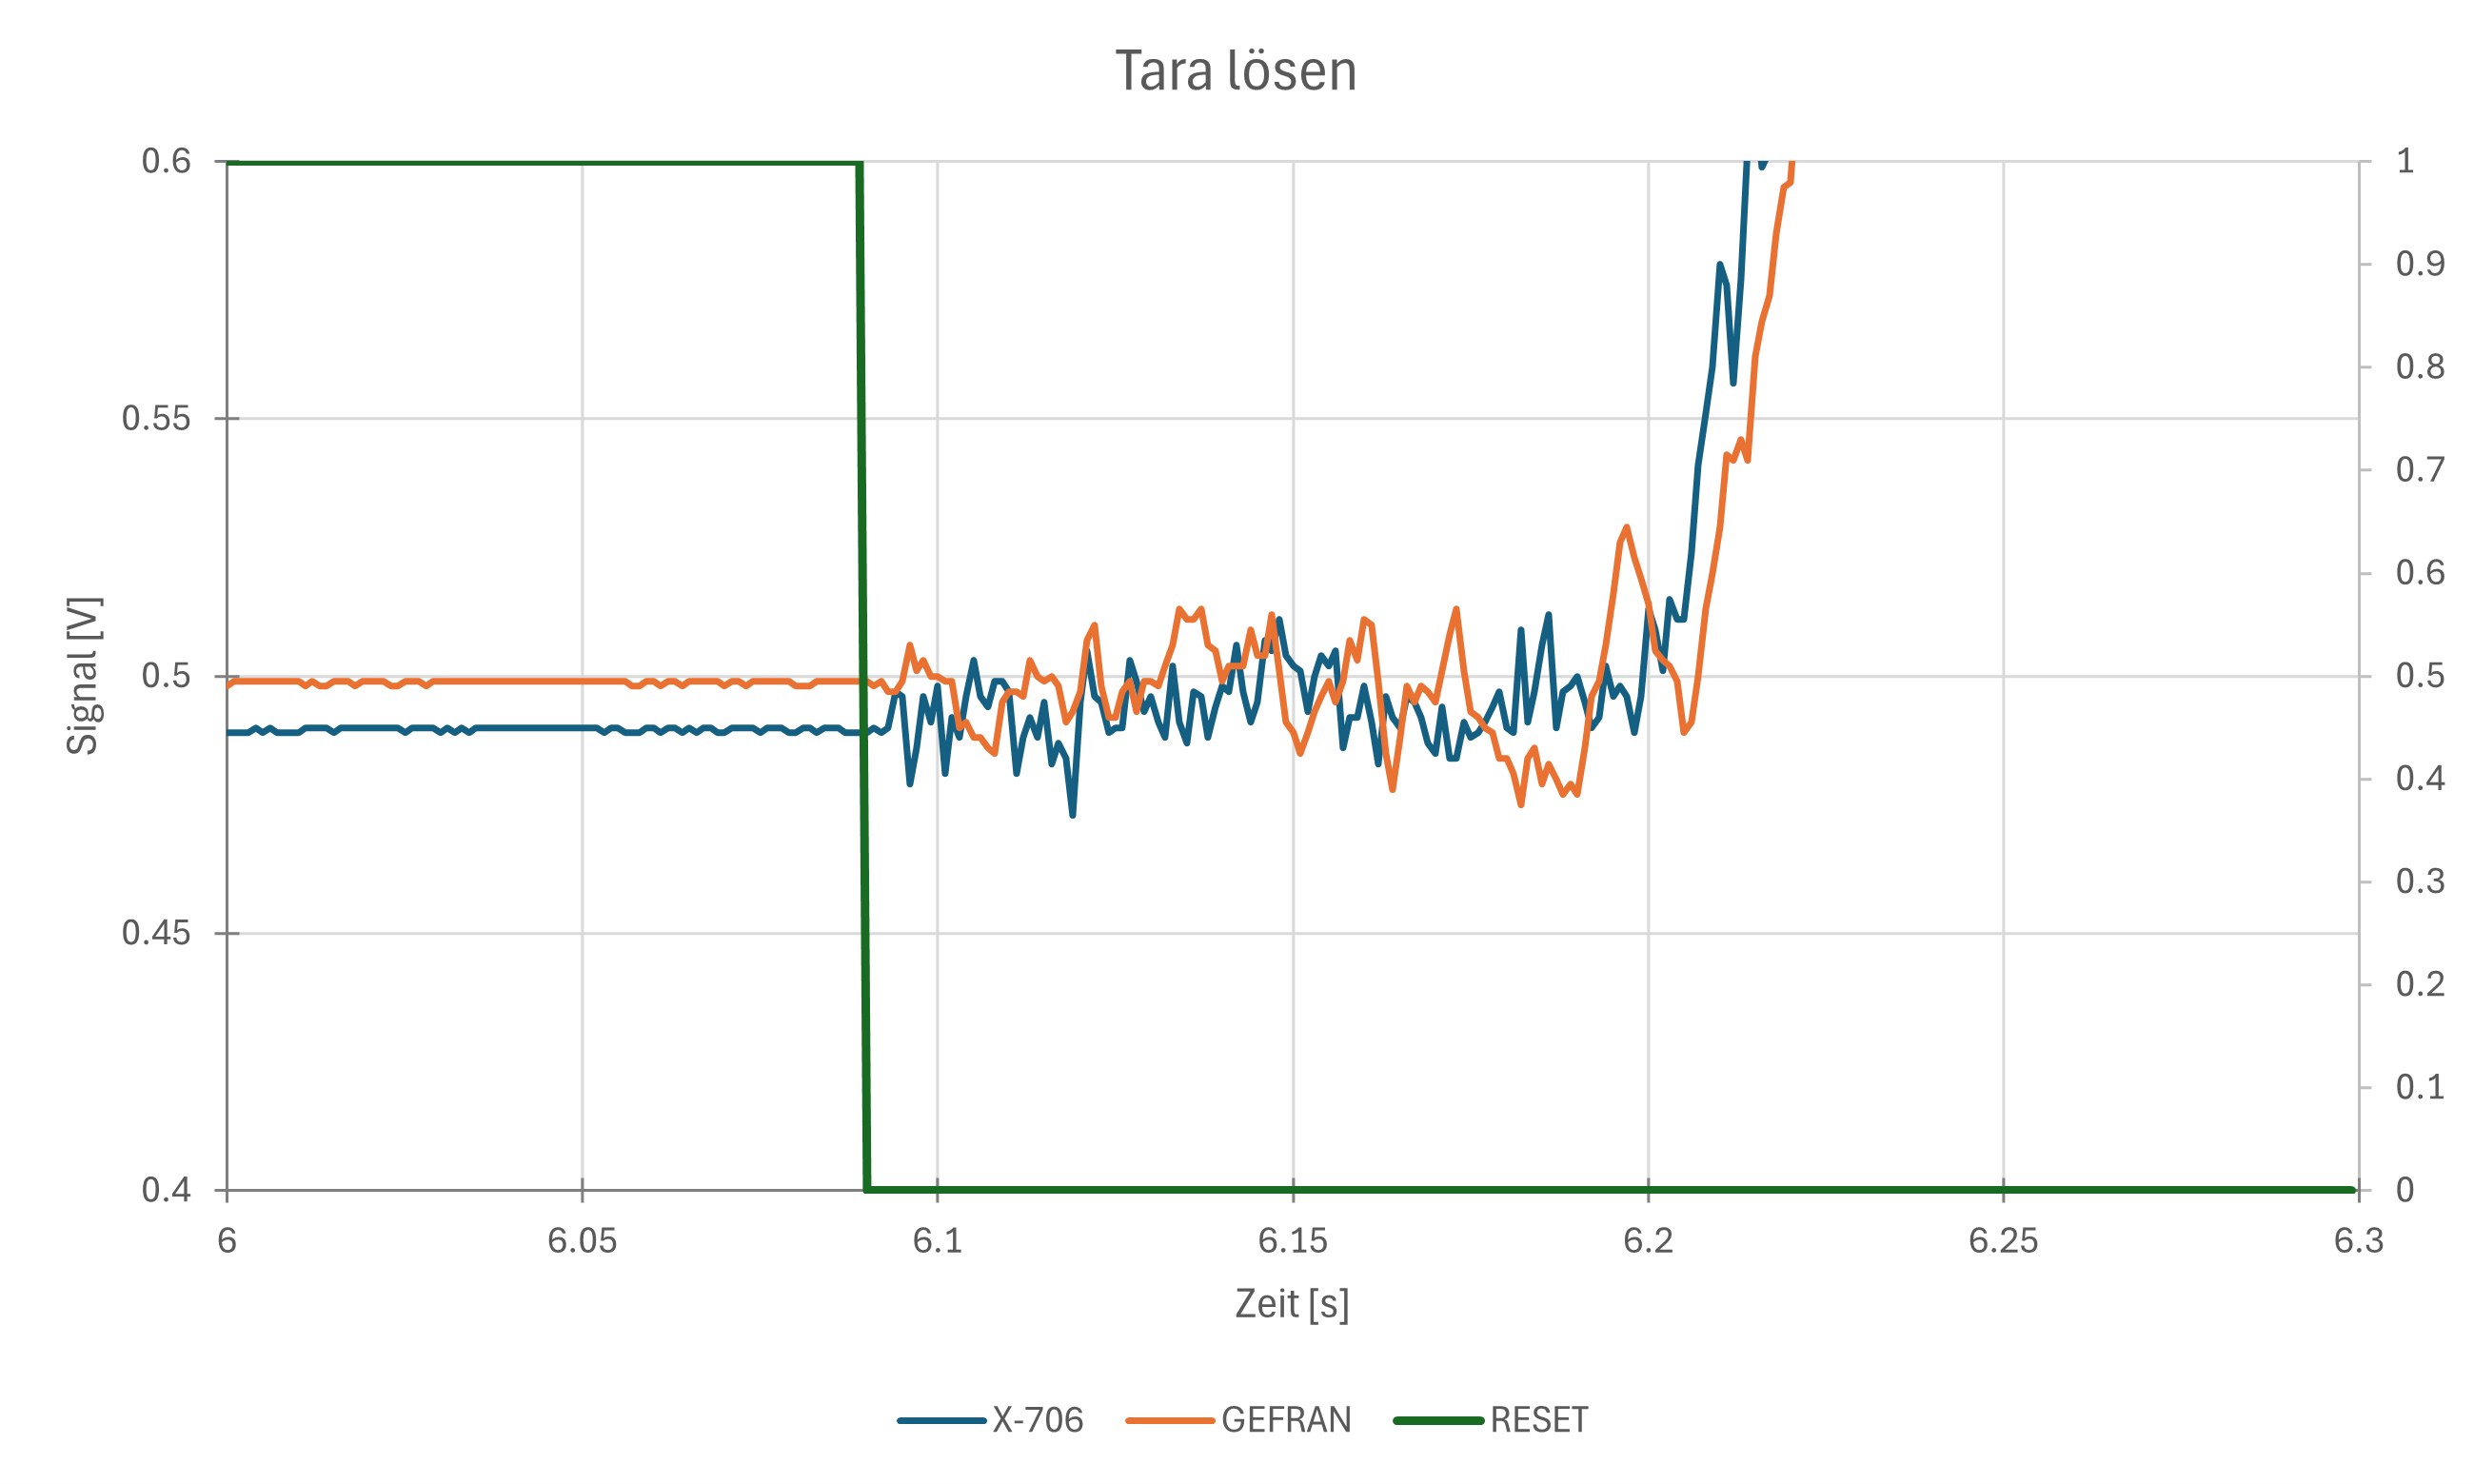
\includegraphics[width=1\linewidth]{imgs/tara_loesen}
	\caption{Signalverlauf beim Lösen des Resets / Tara von 1 auf 0}
	\label{fig:taraloesen}
\end{figure}
Beide Sensoren weisen während anstehendem Reset ein rauscharmes, konstantes Siganl auf, wie es auch in Abschnitt \ref{sec:rauschen} analysiert wurde. Nach dem Lösen des Resets verhalten sich die Sensoren bis zum Bewegungsstart bei ca. 6.2s in guter Näherung identisch.\\
Beim Öffnen der Form verhalten sich die Sensoren ähnlich wie beim Schliessen: der X-706-Sensor zeigt einen etwas weniger geglätteten Signalverlauf, ist aber auch hier etwas schneller bezüglich Signallaufzeit. Es ist zudem zu erkennen, dass der X-706-Sensor beim Beschleunigen betragsmässig kleinere Werte liefert als der GEFRAN-Sensor, beim Verzögern sich dieses Verhältnis jedoch kehrt. Dies ist möglicherweise auf Schlupf bei Lastwechsel zurückzuführen, da der X-706 nur mit 3 von 4 Schrauben befestigt wurde.
\begin{figure}[H]
	\centering
	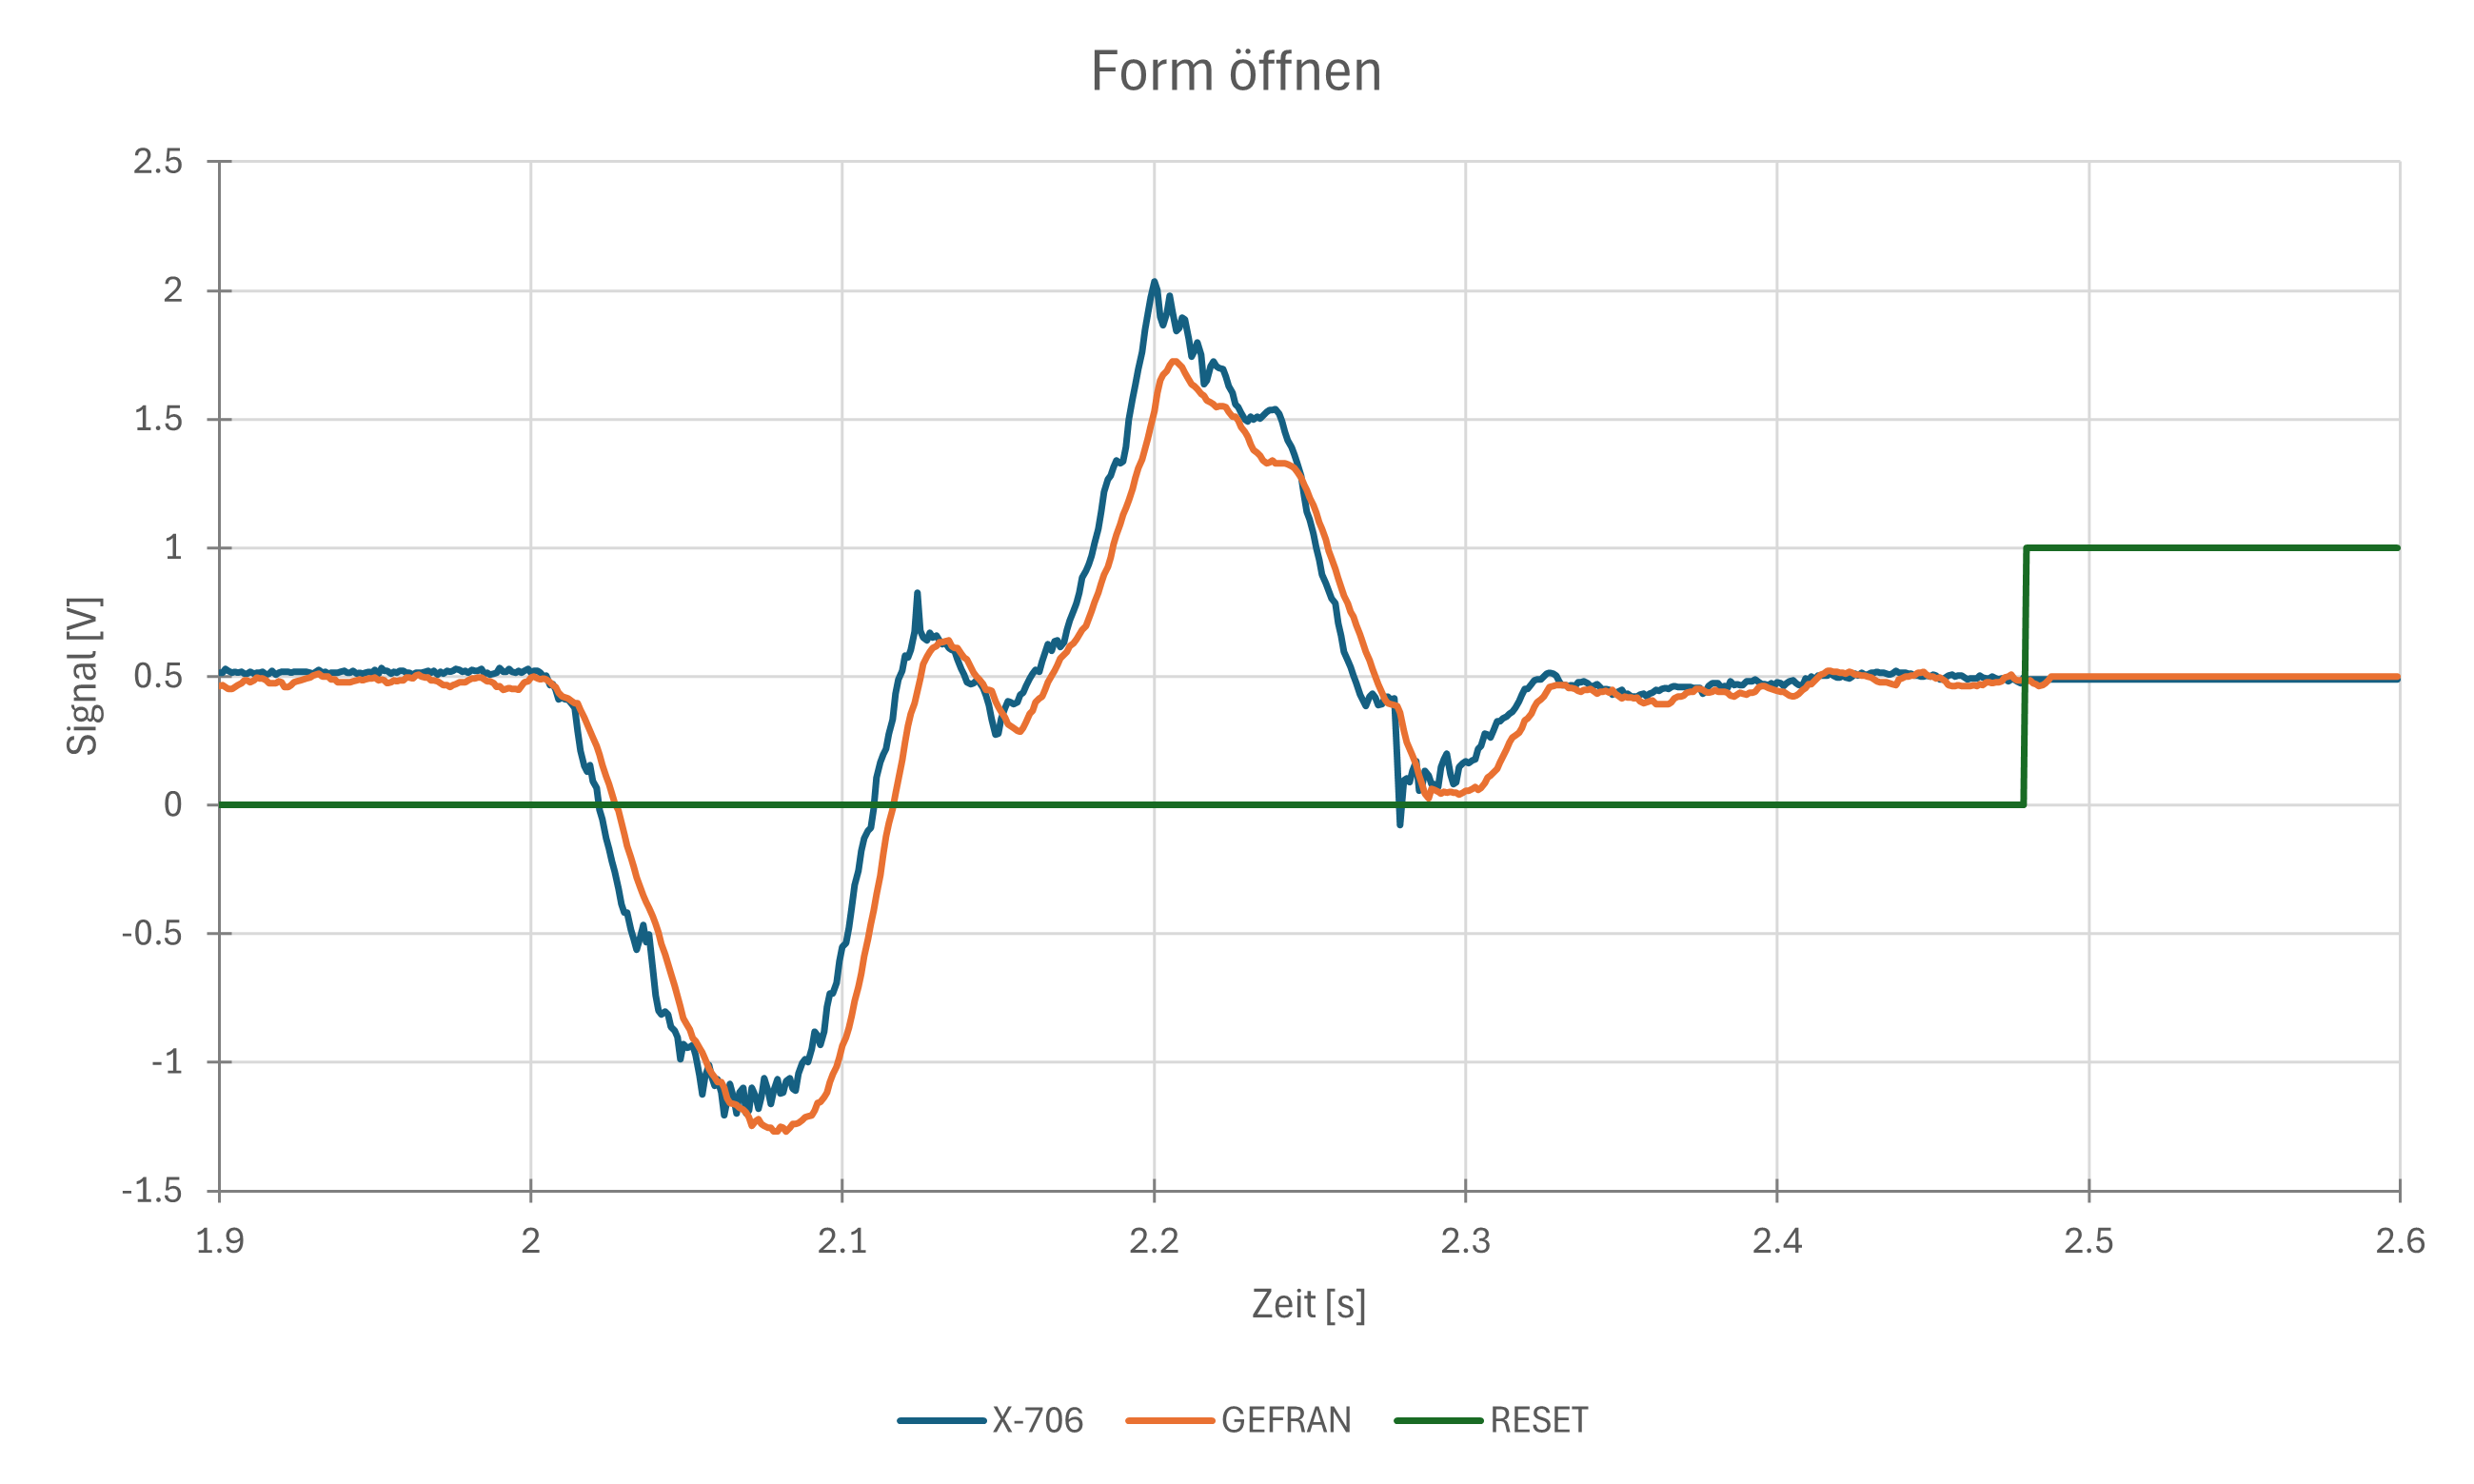
\includegraphics[width=1\linewidth]{imgs/form_oeffnen}
	\caption{Signalverlauf beim Öffnen der Form}
	\label{fig:formoeffnen}
\end{figure}
\section{Vergleich der Kurvenschaaren}
Für den Betrieb der Maschine respektive deren Formschutz wurden zum Schluss noch Kurvenschaaren für beide Sensoren aufgezeichnet sowie ein ''\textit{Kabelbindertest}'' durchgeführt. Insgesamt schneiden beide Sensoren etwa gleich ab, wobei die Schaar des X-706 etwas gebündelter wirkt. Der Ausreiser aus der Schaar über die Toleranzgrenze hinaus wurde durch Einlegen eines Kabelbinders zwischen die Formhälften provoziert. Unter Verwendung des X-706 hat die Maschine etwas früher angehalten als unter Verwendung des GEFRAN-Sensors, was auf die geringere Signalfilterung und die damit verbundenen Signallaufzeit zurückzuführen ist.
\begin{figure}[H]
	\centering
	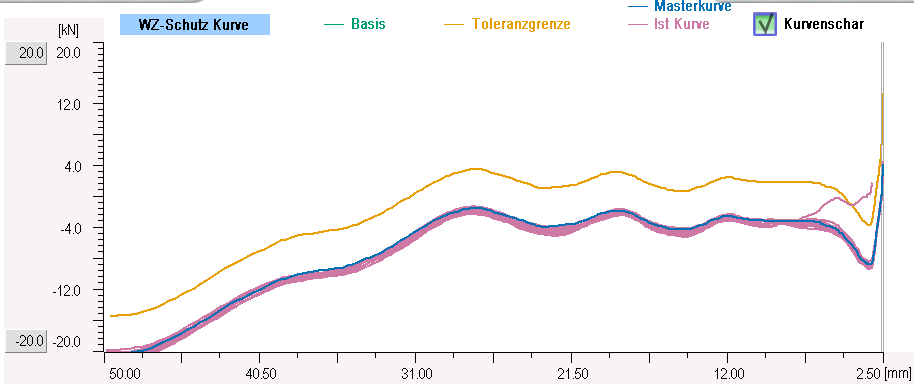
\includegraphics[width=1\linewidth]{imgs/Kurvenschaar_x-706}
	\caption{Kurvenschaar X-706}
	\label{fig:kurvenschaarx-706}
\end{figure}

\begin{figure}[H]
	\centering
	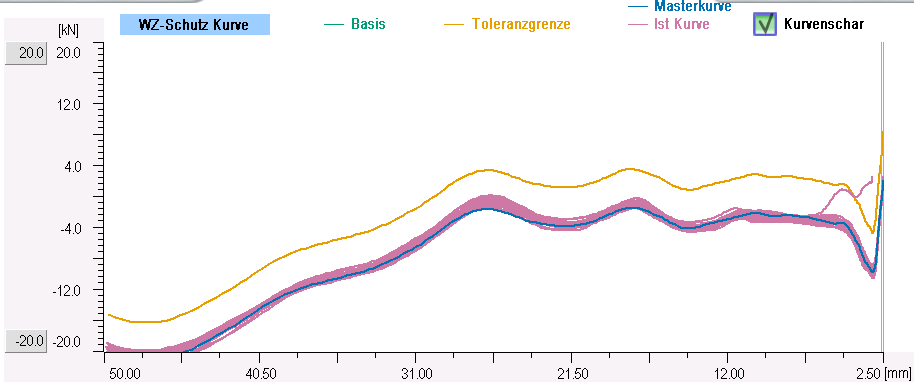
\includegraphics[width=1\linewidth]{imgs/Kurvenschaar_gefran}
	\caption{Kurvenschaar GEFRAN SB46}
	\label{fig:kurvenschaargefran}
\end{figure}
\begin{figure}[H]
	\centering
	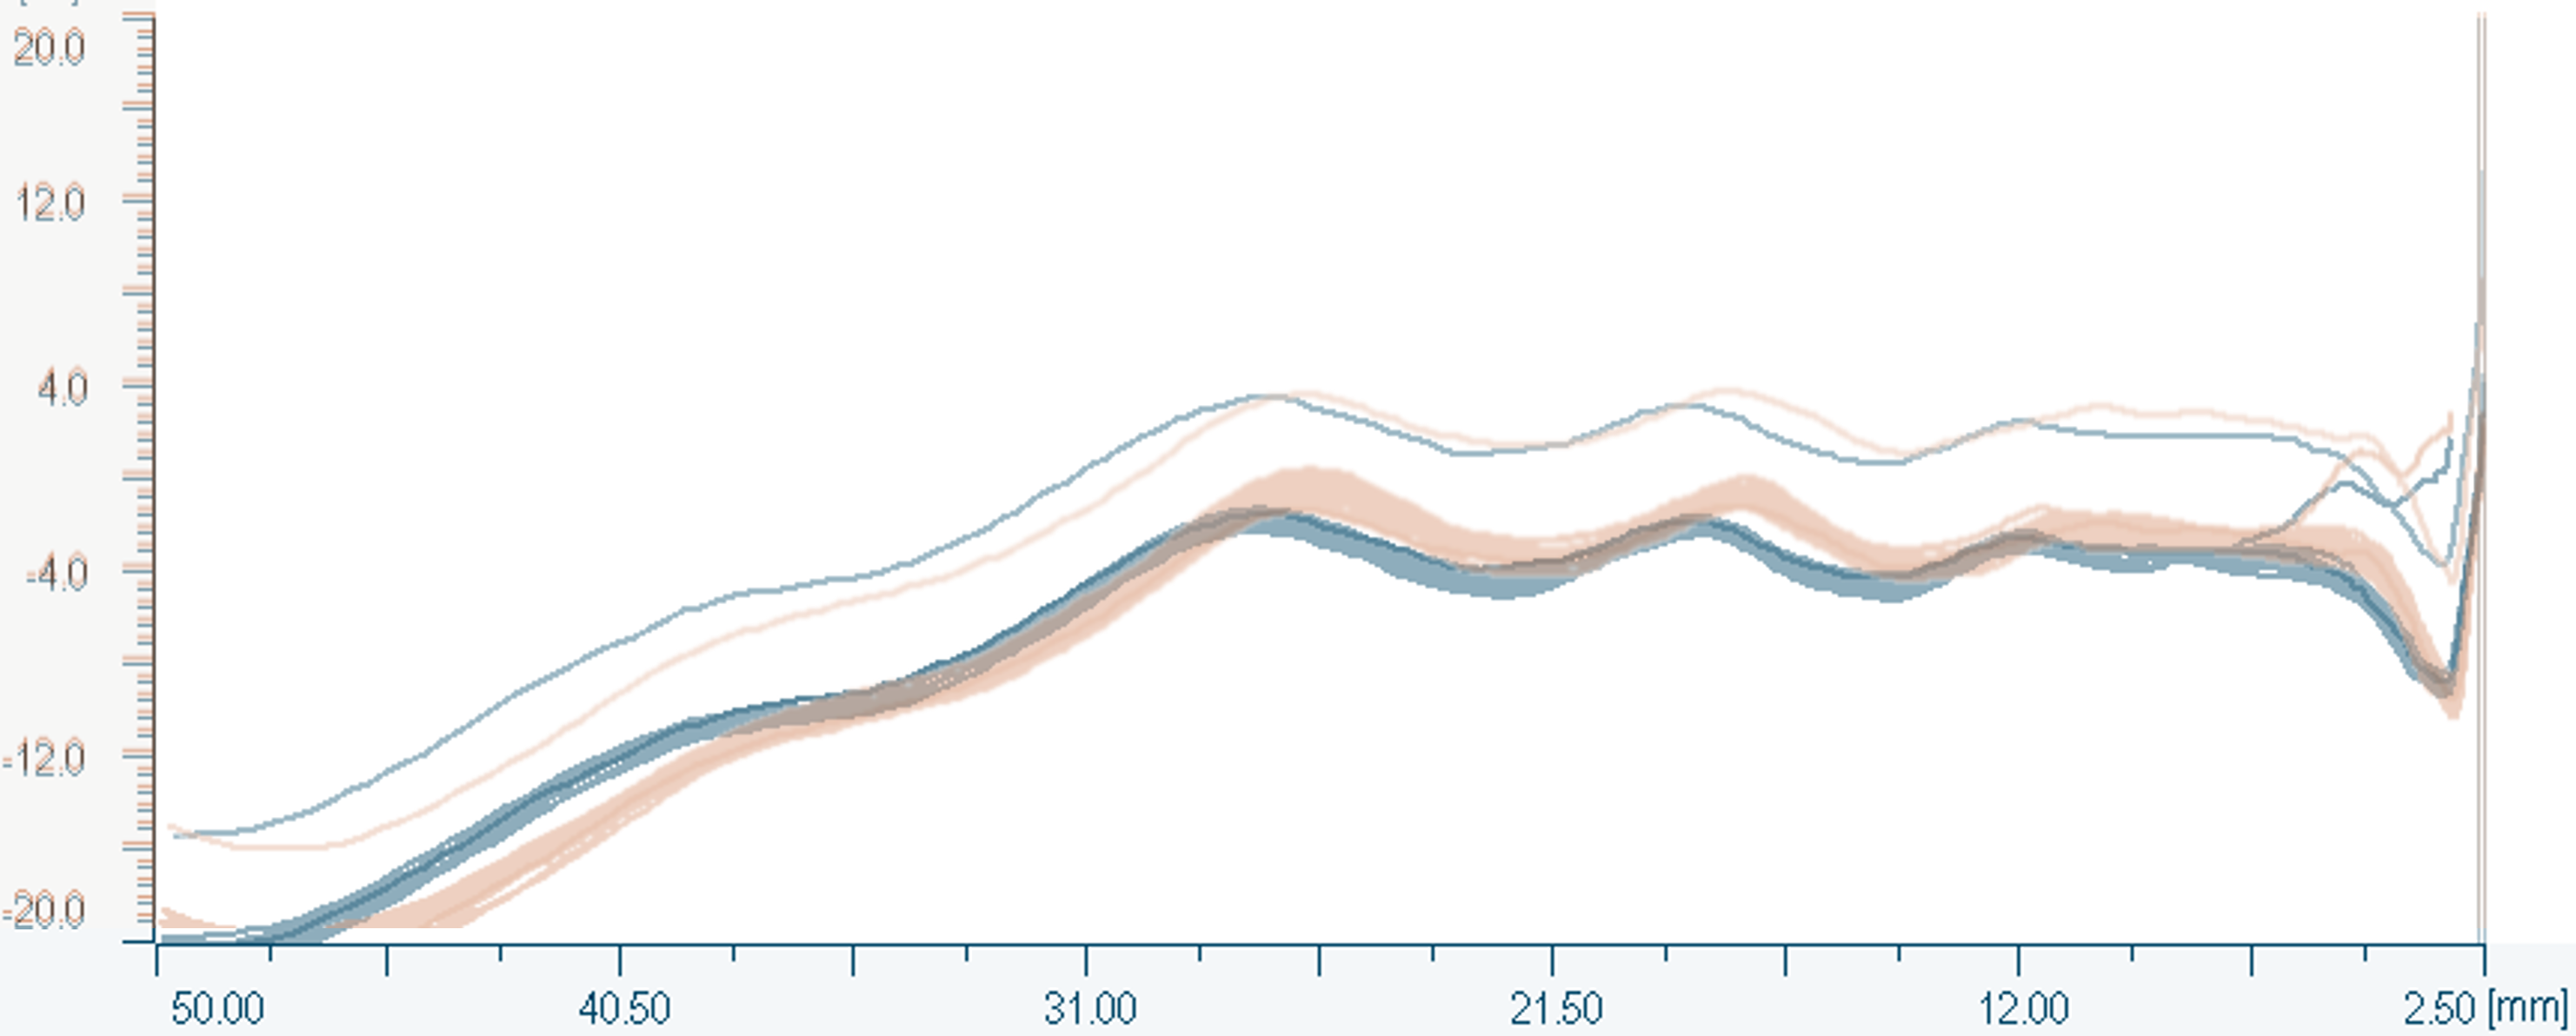
\includegraphics[width=1\linewidth]{imgs/overlaypng}
	\caption[Overlay X-706 (blau) und GEFRAN (orange)]{}
	\label{fig:overlaypng}
\end{figure}
\end{document}
